\documentclass[10pt,letterpaper]{article}
\pdfminorversion=7

% Public flagship preprint.
% Paired-Acquisition Neural Factorization:
% An End-to-End Computational Pathology Pipeline

\usepackage[margin=1in]{geometry}
\usepackage{microtype}
\usepackage{mathptmx}
\usepackage{enumitem}
\usepackage{array,tabularx}
\usepackage{booktabs}
\usepackage{graphicx}
\usepackage{float}
\usepackage{caption}
\usepackage{subcaption}
\usepackage{xurl}
\usepackage[hidelinks]{hyperref}
\usepackage{amsmath,amssymb,amsfonts}
\usepackage{titlesec}
\usepackage{fancyhdr}
\usepackage{lastpage}
\usepackage{placeins}
\usepackage{seqsplit}
\usepackage{xcolor}
\usepackage[numbers,sort&compress]{natbib}

\newcolumntype{Y}{>{\raggedright\arraybackslash}X}

\setlength{\parindent}{0pt}
\setlength{\parskip}{0.54em}
\setlength{\emergencystretch}{3em}
\setlist{nosep,leftmargin=1.5em}
\titleformat{\section}{\large\bfseries}{\thesection.}{0.5em}{}
\titleformat{\subsection}{\normalsize\bfseries}{\thesubsection}{0.5em}{}
\titlespacing*{\section}{0pt}{1.35em}{0.55em}
\titlespacing*{\subsection}{0pt}{1em}{0.35em}
\captionsetup{font=small,labelfont=bf}

\pagestyle{fancy}
\fancyhf{}
\lhead{\small Matthew Vaishnav}
\rhead{\small Paired-Acquisition Neural Factorization}
\cfoot{\small \thepage\ of \pageref{LastPage}}

\begin{document}

\begin{center}
\rule{\linewidth}{4pt}
\vspace{0.22in}

{\LARGE\bfseries Paired-Acquisition Neural Factorization:\\ An End-to-End Computational Pathology Pipeline\par}
\vspace{0.08in}
{\large\bfseries From Scanner-Aware Representations to Whole-Slide and Multi-Institutional Learning\par}

\vspace{0.16in}
{\large Matthew Vaishnav\par}
\vspace{0.08in}
{\normalsize Independent Researcher, Kitchener-Waterloo, Canada\par}
{\normalsize\em Preprint --- 2026-09-04. Research use only; not clinical software.\par}

\vspace{0.22in}
\rule{\linewidth}{1pt}
\end{center}

\begin{center}
\begin{minipage}{0.92\linewidth}
\small
\textbf{Abstract.}
Paired-Acquisition Neural Factorization (PA-NF) is an end-to-end computational pathology research pipeline spanning representation learning, whole-slide neural aggregation, spatial modeling, and multi-institutional learning. The pipeline uses pretrained visual encoders where appropriate, while the paired-factorization methods, slide-level architectures, federated framework, institutional-weighting mechanisms, training and evaluation code, controlled stress experiments, and release infrastructure are developed within the program. The central question is how scanner, site, and institutional variation enters a pathology system and how that information changes as patches become representations, representations become slide predictions, and site-level models become collaborative models.

At the representation stage, the registered SCORPION campaign uses 48 human H\&E slides, 480 aligned tissue regions, five scanners, and 2,400 images. Across 175 completed capacity-matched fits, PA-NF reduced tissue-branch scanner balanced accuracy by 0.3108 relative to an equal-capacity two-branch neural control, with fold/slide bootstrap interval $[-0.3346,-0.2858]$, while same-region retrieval remained within a preregistered 0.02 noninferiority margin and scanner information remained concentrated in an explicit acquisition branch. The frozen objective also transferred across DINOv2, Phikon, and ImageNet ResNet50 feature families. An independent five-scanner canine SCC study provides an external paired-scanner test and a harder boundary: PA-NF produces strong scanner separation, but the corrected fixed five-category comparison does not establish universal superiority over strong simple scanner-removal baselines.

At the whole-slide stage, 10,611 readable PANDA Phikon feature bags support TransnnMIL and federated experiments. Stabilized TransnnMIL remained competitive across 18 full-PANDA runs spanning six learning rates and three seeds, with mean best validation QWK 0.8257 at learning rate $10^{-4}$ and a best recorded run of 0.8455. At the institutional stage, a dominance-aware detector-switch policy on five simulated PANDA sites kept the clean regime essentially unchanged while improving global QWK by $+0.008009$ at 25\% dominant-site corruption and $+0.007482$ at 35\%. A fixed detector calibrated under label-noise stress transferred without retuning to systematic conservative ordinal threshold shift; at 45\% shift it improved global QWK by $+0.01053$, macro-F1 by $+0.01512$, and worst-site QWK by $+0.01290$, with positive 95\% intervals for all three metrics. CAMELYON17/WILDS adds a natural five-center test over 455,954 examples: equal-client weighting improved held-out center accuracy from 0.8312 to 0.9132 on frozen ImageNet features, while dominant-source downweighting reached 0.9322 with source-trained features versus 0.9052 for sample-proportional weighting. PCam provides a complete patch-level benchmark, with a documented run reaching 0.9394 ROC AUC, 0.8526 accuracy, and 0.8507 F1 on the official 32,768-patch test split.

Together, these studies define PA-NF as a connected computational pathology pipeline rather than a single representation model: scanner-aware paired representation learning feeds into whole-slide modeling and then into explicit studies of institutional influence, failure, and adaptive aggregation. The strongest conclusions are comparator-specific: PA-NF has a registered controlled advantage over its equal-capacity neural control on SCORPION; dominance-aware aggregation improves over FedAvg in specified PANDA stress regimes; and alternative source weighting improves held-out-center accuracy in the CAMELYON17 proxy. These results do not constitute clinical validation or a universal state-of-the-art claim.
\end{minipage}
\end{center}

\section{Introduction}

Computational pathology is often divided into separate model problems: patch classification, foundation-model feature extraction, multiple-instance learning, domain robustness, or federated learning. PA-NF is built from the opposite direction. It treats the pathology system as one connected pipeline in which acquisition and institutional effects can enter at several stages and can be amplified as information moves from patches to representations, from representations to slide predictions, and from local models to collaborative models.

The name \emph{Paired-Acquisition Neural Factorization} originated in the representation stage, where exact same-tissue acquisitions expose what changes with scanner while holding the biological region fixed. That paired design remains the foundation of the program, but PA-NF now denotes the full pipeline built around it. Within this manuscript, \emph{PA-NF representation factorization} refers specifically to the tissue/acquisition two-branch model, while \emph{the PA-NF pipeline} refers to the complete computational pathology system.

The pipeline contains four principal authored systems:
\begin{itemize}
\item \textbf{PA-NF representation factorization:} a paired-scanner representation model with explicit tissue-oriented and acquisition-oriented branches, a joint decoder, crossed reconstruction, paired consistency, variance control, and scanner-routing objectives;
\item \textbf{TransnnMIL:} a whole-slide multiple-instance learning architecture family combining transformer-style global correlation modeling with gated aggregation and optional hierarchical, topological, and pruning components;
\item \textbf{PathologyFL:} a pathology-specific federated-learning framework with coordinator/client training, FedAvg/FedProx/FedAdam and custom weighting paths, robustness mechanisms, privacy integrations, monitoring, asynchronous execution, and failure handling;
\item \textbf{FAIR-WEIGHTS-H and dominance-aware aggregation:} institutional weighting and detector-switch mechanisms that test when sample-count authority should yield to cross-site evidence, uncertainty, and reliability signals.
\end{itemize}

These systems share a common experimental layer. PCam provides patch-level training and evaluation. SCORPION and multi-scanner canine SCC provide exact paired acquisitions across five scanners. PANDA provides 10,611 readable slide-level Phikon feature bags for whole-slide modeling and simulated institutional stress. CAMELYON17/WILDS supplies 455,954 examples across five centers for natural center-shift studies. Controlled latent-factor generators provide ground truth for mechanism questions that cannot be observed directly in pathology data.

The central scientific hypothesis is that scanner and site variation should not be treated as a single preprocessing nuisance. A scanner shortcut can be encoded in a patch representation, attended to by a slide model, and then amplified through institutional aggregation. Conversely, institutional reweighting can change which representation failures dominate the global model. PA-NF therefore studies the transitions between these levels rather than optimizing them in isolation.

The main contributions of this paper are: (i) a registered paired-acquisition representation result on SCORPION with an equal-capacity neural control and cross-backbone transfer; (ii) an independent multi-scanner canine study that tests the limits of the representation claim against strong simple corrections; (iii) an implemented whole-slide architecture and full-PANDA stabilization study; (iv) a custom federated pathology stack with a dominance-aware detector that improves over FedAvg in controlled PANDA failure regimes and transfers without retuning to systematic ordinal shift; and (v) a CAMELYON17 held-out-center study showing that source influence and source sample count are not interchangeable.

The goal is not to collapse these experiments into one leaderboard. Each dataset answers a different question at a different level of the pipeline. The result is a single research system with several experimentally linked components, not a claim that one metric or one model dominates all of computational pathology.

\section{Research-program overview}

The program is organized as three primary neural aggregation levels plus the
benchmark and provenance infrastructure that connects them.

\begin{enumerate}
\item \textbf{Level I --- Representation formation.} How patch and
  foundation-model representations encode tissue, scanner, stain, acquisition
  workflow, site or center, region identity, and dataset artifacts. Principal
  research lines: PCam patch foundation; paired-scanner and paired-acquisition
  research; Paired-Acquisition Neural Factorization; SCORPION; multi-scanner
  canine SCC; scanner and center subspaces; centroid/QR, PCA, paired-linear,
  adversarial, and broken-pair controls; and synthetic identifiability and
  capacity-allocation studies.
\item \textbf{Level II --- Whole-slide aggregation.} How patch representations
  are aggregated into slide predictions. Principal research line: TransnnMIL and
  all of its implemented architectural families (canonical dual-branch,
  three-branch v2, branch-token fusion, hierarchical pooling, topology branch,
  adaptive pruning, graph caching).
\item \textbf{Level III --- Institutional aggregation.} How multi-institution
  updates, validation priorities, contribution signals, and safety constraints
  are aggregated. Principal research lines: PathologyFL; FAIR-WEIGHTS-H;
  institutional weighting; dominant-site stress testing; site imbalance;
  ordinal-grading shift; corruption and label-noise stress; detector behavior;
  client heterogeneity, dropout, and stragglers; communication accounting;
  secure aggregation; differential-privacy support; Byzantine or anomaly
  monitoring; and CAMELYON17 held-out-center and center-weighting studies.
\end{enumerate}

The three levels are connected by a shared evaluation and accountability
framework, and by shared frozen feature inputs (DINOv2, Phikon
\cite{filiot2023phikon}, ImageNet ResNet): scanner leakage, center leakage, descriptive task accessibility,
region retrieval, whole-slide aggregation, institutional influence, fairness
constraints, robustness, provenance, and claim validity are audited with the same
fail-closed discipline at every level. PCam provides the patch-level benchmark
foundation; PANDA provides the whole-slide benchmark; CAMELYON17 provides the
multi-center benchmark; and the provenance system binds every active claim to an
immutable artifact.

The unifying thesis is that computational-pathology neural systems aggregate
information at several levels --- patches into representations, patch instances
into whole-slide predictions, and institutional updates into collaborative
models --- and at each level nuisance variation, shortcut signals, optimization
failures, and institutional imbalance can be preserved or amplified. This program
develops the neural architectures, paired-data designs,
institutional-weighting protocols, stress tests, and provenance controls for
auditing and improving those aggregation stages.

\begin{equation}
\begin{aligned}
h_{r,s} &= E_{\omega}(x_{r,s}), \\
\mathcal{F}_{\mathrm{pair}}:\ \{h_{r,s}\}_{s\in\mathcal{S}_{r}}
&\longmapsto \left(z^{\mathrm{tissue}}_{r,s},z^{\mathrm{acq}}_{r,s}\right), \\
\mathcal{A}_{\mathrm{slide}}:\ \{(z_{k,j},p_{k,j})\}_{j\in\mathcal{B}_{k}}
&\longmapsto \widehat y_{k}, \\
\mathcal{A}_{\mathrm{site}}:\ \{(\Delta\theta_{i}^{(t)},w_{i}^{(t)})\}_{i\in\mathcal{I}_{t}}
&\longmapsto \theta^{(t+1)}, \\
\mathcal{P}_{\mathrm{PA\text{-}NF}}
&= \mathcal{A}_{\mathrm{site}}\circ\mathcal{A}_{\mathrm{slide}}\circ\mathcal{F}_{\mathrm{pair}}\circ E_{\omega}.
\end{aligned}
\label{eq:program}
\end{equation}

\noindent Here $E_{\omega}$ is a frozen or task-trained visual encoder, $\mathcal{F}_{\mathrm{pair}}$ is the paired-acquisition representation stage, $\mathcal{A}_{\mathrm{slide}}$ is whole-slide aggregation (TransnnMIL and matched MIL baselines), and $\mathcal{A}_{\mathrm{site}}$ is institutional aggregation (PathologyFL, FedAvg-family baselines, and dominance-aware weighting). Spatial coordinates $p_{k,j}$ are optional inputs to the slide stage for spatial and topology experiments.

\begin{figure}[!htbp]
\centering
\small
\caption{Publication-portfolio map. The flagship foundations manuscript frames
the program; focused papers A--D carry scoped evidence. Release order is
flagged by evidence maturity.}
\label{fig:portfolio}
\resizebox{\columnwidth}{!}{\begin{tabular}{lll}
\toprule
Component & Scope & Release readiness \\
\midrule
Flagship foundations manuscript & all three levels + audit & internal-review ready \\
Focused Paper A (PA-NF) & representation; negative increment; Layer-2 & corrected evidence ready \\
Focused Paper B (TransnnMIL) & whole-slide architecture & pending matched reruns \\
Focused Paper C (FL/FAIR-WEIGHTS-H) & institutional; infrastructure & after implementation completion \\
Focused Paper D (provenance) & audit system & portfolio decision \\
\bottomrule
\end{tabular}}
\end{figure}


\noindent\textbf{Evidence-maturity discipline.} Throughout, the manuscript keeps
four distinct categories separate: \emph{implemented architecture} (binds to
source and tests), \emph{corrected empirical evidence} (binds to immutable
result artifacts), \emph{negative or mixed results} (reported directly), and
\emph{pending controlled validation} (labeled pending). No component is implied
to have the same evidence maturity as any other.

\section{Benchmark and engineering foundation}
\begin{figure}[!htbp]
\centering
\small
\caption{Dataset and evidence-boundary map (verified at inventory time).}
\label{fig:datasets}
\resizebox{\columnwidth}{!}{\begin{tabular}{llll}
\toprule
Dataset & Scale & Endpoints & Evidence boundary \\
\midrule
PCam & 96$\times$96 patches; 32,768 test & binary tumor patch & patch benchmark; not clinical \\
SCORPION & 48 slides, 480 regions, 5 scanners, 2,400 patches & scanner, retrieval, geometry & no category labels \\
Canine SCC & 4,025 patches, 7 categories, 5 scanners & corrected 5-category, scanner, retrieval & descriptive categories; not clinical \\
PANDA & 10,611 readable Phikon slides, ISUP 0--5 & QWK, institutional stress & simulated sites; no real mapping \\
CAMELYON17 & 455,954 patches, 5 centers & held-out-center accuracy, center leakage & centralized frozen-feature proxy; not full FL \\
\bottomrule
\end{tabular}}
\end{figure}


The program is built on patch-level benchmark and evaluation infrastructure that
establishes deterministic data handling, evaluation methodology, calibration and
uncertainty analysis, and federated smoke validation.

\subsection{PCam patch benchmark}

PCam (PatchCamelyon) \cite{veeling2018rotation,pcam2018kaggle} is used as a
patch-level engineering and evaluation
benchmark: a binary tumor-detection task over 96$\times$96 RGB patches. The
implementation includes a dataset API, binary classification head, ResNet and
transformer feature extractors, full-config training, full-test evaluation with
ROC AUC / accuracy / F1 and bootstrap confidence intervals, stratified
cross-validation, threshold operating-point analysis, and failure-asymmetry
analysis. Federated smoke and heterogeneity benchmarks use real PCam patches
split into simulated sites to exercise weighting strategies.

\subsection{What PCam establishes}

The strongest documented PCam result is a single trained run with ROC AUC
0.9394, accuracy 0.8526, and F1 0.8507 on the official 32{,}768-patch test
split, with patch-level bootstrap confidence intervals. This is a documented
observed run; the raw artifacts are not tracked in the repository. PCam
establishes:

\begin{itemize}
\item a working patch-level training and evaluation pipeline;
\item bootstrap and evaluation infrastructure with tests;
\item a foundation for later federated and whole-slide infrastructure.
\end{itemize}

\subsection{What PCam does not establish}

PCam does not establish clinical validation, diagnostic performance,
patient-level or slide-level endpoints, external generalization, statistical
superiority over unrelated published models, or calibration at a clinically
meaningful operating point. The 5-fold cross-validation tables in documentation
are projected (the cross-validation run is paused), not observed. The
threshold-optimization study is retrospective and was withdrawn as
confirmatory or deployment evidence. No selected threshold is recommended for
inference or deployment. The current status is \emph{patch-level engineering
and evaluation benchmark only}, and clinical and deployment prohibitions are
enforced by the authoritative claim boundary.

\section{Stage I: paired-acquisition representation learning}
\begin{figure*}[!t]
\centering
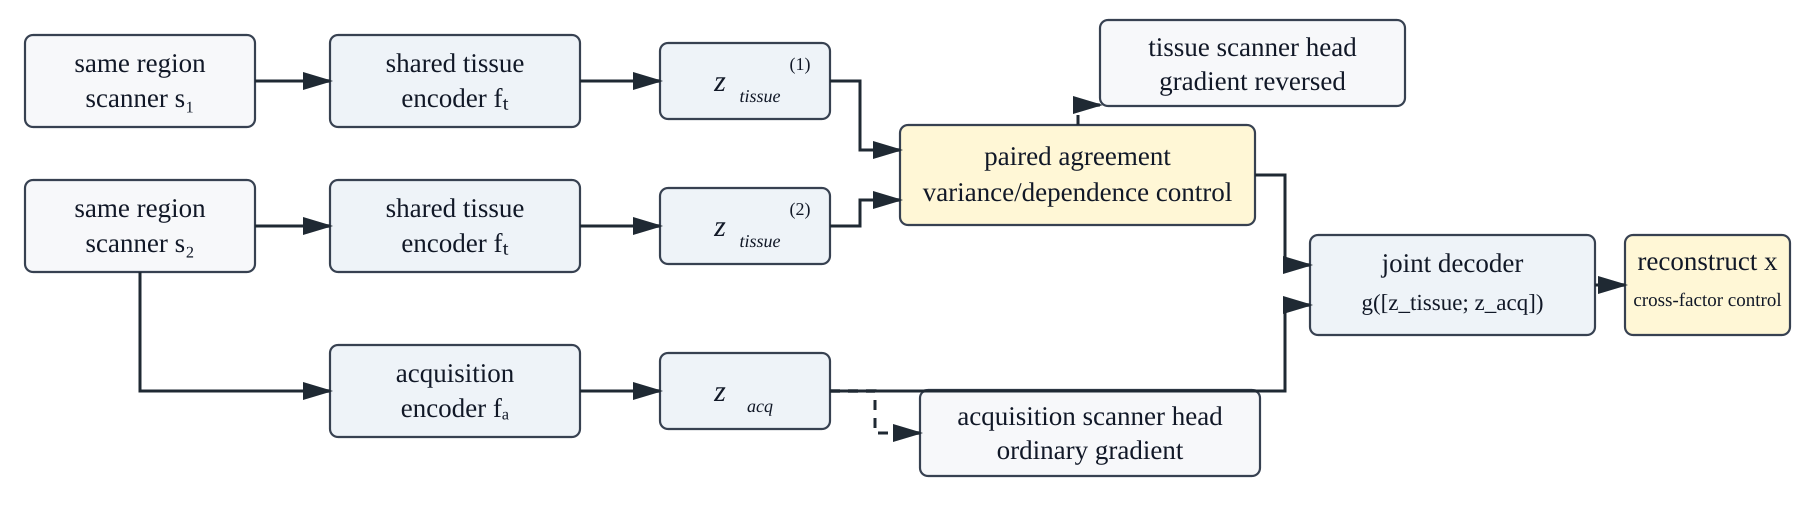
\includegraphics[width=\textwidth]{figures/pa_nf_architecture.pdf}
\caption{Paired-Acquisition Neural Factorization routes matched views of the
same tissue region through a shared tissue-oriented encoder and an explicit
acquisition branch. Paired agreement, variance/dependence control, a
gradient-reversed tissue scanner head, an ordinary acquisition scanner head,
and joint decoding structure how scanner-associated information is allocated.
The diagram describes the implemented architecture; the corrected empirical
boundary remains partial structured separation rather than pure factors,
complete scanner invariance, or clinical utility.}
\label{fig:panf}
\end{figure*}


The representation stage asks whether matched acquisitions can provide a useful supervisory signal for allocating scanner-associated variation without simply erasing the representation. For a region observed under several scanners, PA-NF learns a tissue-oriented branch $b_{r,s}$ and an acquisition-oriented branch $a_{r,s}$, with crossed reconstruction, same-region consistency, acquisition prediction, dependence control, and variance regularization. Tissue or diagnostic category labels are not required to construct the paired objective.

\subsection{Registered SCORPION capacity-matched experiment}
The primary human paired-scanner experiment uses SCORPION \cite{ryu2023scorpion}: 48 original H\&E slides, ten aligned regions per slide, and five scanner views per region, for 480 biological regions and 2,400 images. The registered capacity-matched campaign contains seven variants, five folds, and five seeds, for 175 completed fits. Its primary comparator is an equal-capacity two-branch neural control without the scanner-routing objectives.

\begin{table*}[t]
\centering
\caption{Primary registered SCORPION comparison: PA-NF minus the equal-capacity two-branch neural control. Negative tissue scanner balanced accuracy is favorable; retrieval is judged against the registered 0.02 noninferiority margin.}
\label{tab:scorpion_primary}
\small
\begin{tabular}{lrrl}
\toprule
Metric & Mean difference & 95\% fold/slide interval & Result \\
\midrule
Tissue scanner balanced accuracy & $-0.3108$ & $[-0.3346,-0.2858]$ & Lower scanner recoverability \\
Mean same-region top-1 retrieval & $+0.00004$ & $[-0.00009,+0.00026]$ & Noninferior \\
Mean paired cosine & $+0.03639$ & $[+0.03355,+0.03954]$ & Positive geometry contrast \\
Worst paired cosine & $+0.03557$ & $[+0.03167,+0.04064]$ & Positive geometry contrast \\
Acquisition scanner balanced accuracy & $+0.1180$ & $[+0.1003,+0.1358]$ & Stronger explicit scanner routing \\
\bottomrule
\end{tabular}
\end{table*}

The key result is the joint pattern: tissue-branch scanner recovery falls substantially relative to the capacity-matched neural control, same-region retrieval remains inside the predefined noninferiority margin, and scanner information becomes more recoverable from the acquisition branch. This supports a controlled comparative advantage on the registered SCORPION structured-separation objective. Because SCORPION does not supply a validated biological-category endpoint for these regions, the result is a representation result rather than a disease-biology claim.

\subsection{Cross-backbone transfer}
The frozen objective was transferred without backbone-specific tuning across DINOv2-Base, pathology-native Phikon, and ImageNet ResNet50 representations. In the transfer study, PA-NF reduced scanner recoverability in the tissue branch while retaining near-saturated same-region retrieval across all three feature families. Averaging the two unseen feature families within the same 48 SCORPION slides gave a scanner-probe difference of $-0.4019$ with interval $[-0.4145,-0.3895]$. The acquisition branch remained strongly scanner informative. This result shows that the paired objective is not tied to one visual encoder, although the registered DINOv2 capacity-matched campaign remains the primary controlled comparison.

\subsection{Independent multi-scanner canine SCC study}
The external paired-scanner study uses 44 canine cutaneous squamous-cell-carcinoma biological samples digitized on five scanners. After geometry qualification, 805 complete five-view regions are available. The corrected evaluation fixes five descriptive tissue categories---Dermis, Epidermis, Inflammation/Necrosis, SCC, and Subcutis---and uses biological-sample-blocked folds, fit-only standardization, and same-region/same-sample exclusions in nearest-neighbour candidate pools.

\begin{table*}[t]
\centering
\caption{Corrected five-fold canine SCC representation comparison. Category balanced accuracy is descriptive; lower scanner balanced accuracy and higher retrieval are favorable.}
\label{tab:canine_corrected}
\small
\begin{tabular}{lrrrr}
\toprule
Representation & Category BA & Scanner BA & Overall retrieval & Worst-pair retrieval \\
\midrule
Original frozen features & 0.4439 & 0.8635 & 0.8724 & 0.7613 \\
Centroid/QR scanner projection & 0.4414 & 0.3278 & 0.9099 & 0.8196 \\
Paired linear scanner transform & 0.4422 & 0.3687 & 0.9022 & 0.8283 \\
PCA component removal & 0.3949 & 0.8157 & 0.9197 & 0.8512 \\
PA-NF tissue branch B32 & 0.4331 & 0.2996 & 0.7192 & 0.5848 \\
PA-NF tissue branch B64 & 0.4255 & 0.3486 & 0.7707 & 0.6345 \\
\bottomrule
\end{tabular}
\end{table*}

The canine experiment establishes an important boundary around the SCORPION result. PA-NF B32 attains the lowest mean scanner balanced accuracy in the corrected table, but strong centroid/QR and paired-linear corrections preserve higher retrieval while retaining similar descriptive category accuracy. Under the registered three-axis rule, neither B32 nor B64 establishes a universal neural feature-space increment over every simple baseline. Increasing the tissue bottleneck from 32 to 64 dimensions increases overall retrieval by $+0.0515$ and scanner recoverability by $+0.0489$, while corrected category balanced accuracy changes by $-0.0076$ with an interval crossing zero.

This is not a contradiction with the SCORPION controlled result. The two experiments use different comparators and endpoints. SCORPION establishes a bounded advantage over an equal-capacity neural control on the registered structured-separation objective; the canine study shows that broader scanner correction has a harder frontier in which strong linear methods remain competitive.

\subsection{Pair integrity and information routing}
Broken-pair controls provide a direct test of whether scanner suppression alone explains the result. Region- and sample-shuffled pairings can reduce scanner probe accuracy as much as, or more than, true same-region pairs, but they degrade same-region agreement and retrieval. Correct pairing therefore constrains what the system preserves rather than merely teaching it to confuse a scanner classifier.

The explicit acquisition branch is equally important. Scanner information remains strongly recoverable there, so the intended operation is allocation rather than wholesale deletion. The observed separation is partial and estimator-dependent: low linear scanner recoverability is not information-theoretic independence, and same-region retrieval is not a clinical or diagnostic endpoint.

\section{Level II: TransnnMIL whole-slide aggregation}
\begin{equation}
\begin{aligned}
H_k &= [h_{k,1},\ldots,h_{k,n_k}]^{\top}, \\
b_A &= \mathcal{M}_{\mathrm{Trans}}(H_k),
& b_B &= \mathcal{M}_{\mathrm{att}}(H_k), \\
T_k &=
\begin{bmatrix}
P_A b_A \\
P_B b_B
\end{bmatrix}
\in\mathbb{R}^{2\times d}, \\
Q_k &= T_kW_Q,
& K_k &= T_kW_K,
& V_k &= T_kW_V, \\
A_k &= \operatorname{softmax}\!\left(\frac{Q_kK_k^{\top}}{\sqrt{d_h}}\right), \\
\widetilde T_k &= \operatorname{LN}\!\left(T_k+A_kV_k\right), \\
z_k &= \frac{1}{2}\mathbf{1}^{\top}\widetilde T_k,
& \widehat y_k &= C_{\eta}(z_k).
\end{aligned}
\label{eq:transnnmil}
\end{equation}

\begin{equation}
\mathcal{B}_{\mathrm{v2}}
\subseteq
\left\{
\mathcal{M}_{\mathrm{Trans}},
\mathcal{M}_{\mathrm{att}},
\mathcal{M}_{\mathrm{hier}},
\mathcal{M}_{\mathrm{graph}}
\right\},
\qquad
T_k=\operatorname{stack}\!\left(\{P_jb_j:j\in\mathcal{B}_{\mathrm{v2}}\}\right).
\label{eq:transnnmil-v2}
\end{equation}


Whole-slide prediction requires aggregating tens of thousands of patch
representations into a single slide-level decision. This is the second primary
aggregation level. The program's contribution here is TransnnMIL, a multibranch
whole-slide neural aggregation architecture family. The architecture is an
authored and implemented contribution; its corrected matched-control superiority
evaluation is pending. Historical performance numbers produced by a defective
execution path are withdrawn and are never used as repaired-model evidence.

\subsection{Verified architectural families}

The implementation lives in \texttt{src/models/transnnmil/} and is described
here from the code, not from stale marketing prose. The verified families are:

\begin{itemize}
\item \textbf{Canonical TransnnMIL} (\texttt{transnnmil.py}): a dual-branch
  model with a TransMIL-style global-correlation branch
  (\texttt{src/models/mil/transmil.py}, after TransMIL \cite{shao2021transmil})
  and an nnMIL-style gated-attention
  branch (\texttt{src/models/mil/nnmil.py}, after attention-based
  multiple-instance learning \cite{ilse2018attention}). The repaired model fuses the
  branches by \emph{self-attention over explicit branch tokens}: the two
  projected branch representations are stacked and attended
  (\texttt{branch\_token\_fusion.py}), replacing the withdrawn one-query
  one-key cross-attention path that was query-invariant. Explicit branch
  representations are implemented and tested.
\item \textbf{TransnnMILv2} (\texttt{transnnmil\_v2.py}): a three-branch
  variant (TransMIL + hierarchical pooling + topology), a two-branch variant
  with AB/AC/BC ablations, and explicit branch-token fusion. No empirical
  results exist for these variants; numbers in design documentation are
  explicitly projected, not observed.
\item \textbf{Fusion controls} (\texttt{branch\_token\_fusion.py},
  \texttt{transnnmil\_branch\_token.py}): learned branch-attention, concat, and
  gate fusion operators, aligned to the repaired canonical branches. Implemented
  and tested, but \emph{planned controls} with no recorded results yet.
\item \textbf{Hierarchical spatial pooling} (\texttt{hierarchical\_pooling.py}):
  learnable cluster centers, region attention/mean/max pooling, and region
  transformers. Implemented and tested; a synthetic-MIL ablation exists, and a
  real-data benchmark is planned. Enabled in the canonical model only when
  requested (default off); PANDA runs did not enable it.
\item \textbf{Topology or graph branch} (\texttt{topology\_branch.py}): k-NN
  graph construction and GNN layers (GATv2, GraphSAGE, GIN). Implemented and
  tested. \emph{Historical topology results are withdrawn}: the old forward pass
  created an unregistered random projection. The repaired model registers the
  projection; a post-repair rerun does not yet exist.
\item \textbf{Adaptive pruning} (\texttt{adaptive\_pruning.py}): importance
  scoring and adaptive pruning. Implemented and tested, but disabled in
  TransnnMILv2 pending a proper batched implementation; no results.
\item \textbf{Graph caching and coordinate-aware processing}
  (\texttt{graph\_cache.py}): HDF5 k-NN graph precompute and cache. Implemented
  and tested; no training result.
\end{itemize}

\subsection{Branch-token fusion mechanism}

The corrected fusion is the technical heart of the canonical model. Each branch
produces a sequence of patch-level representations; the branch representations
are projected to a fixed token dimension and stacked into an explicit branch-token
sequence $T \in \mathbb{R}^{2 \times d}$, one token per branch. A multi-head
self-attention over $T$ computes the fused slide representation as a learned
interaction between the two branch tokens, and the attended tokens are
mean-pooled before the classifier head. This fixes the historical defect: the
old one-query/one-key cross-attention used a single query token against a single
key, so the softmax over one position was identically $1$ and the fusion was
\emph{query-invariant} --- it could not weight the branches at all. The repaired
design gives the fusion genuine branch-interaction capacity, and regression tests
require output sensitivity and gradient flow to both branches
(\texttt{tests/models/test\_transnnmil\_canonical\_fusion.py}). The incremental
contribution of this fusion relative to concat and gate controls is \emph{not yet
measured}; that is exactly the pending matched-control evaluation. A full
per-component implementation/test/result matrix is in the supplement.

\subsection{PANDA training infrastructure and feature bags}

The PANDA training infrastructure uses a verified Phikon 768-dimensional feature
bag manifest (10{,}611 readable slide feature files; 8{,}488 train and 2{,}123
validation rows) with \texttt{train\_panda\_transnnmil\_baseline.py}. Stability
grids across learning rates and seeds show best validation QWK in the
0.812--0.826 range, and ablation runs exist. These numbers are
\emph{preliminary and pending}: they are not yet matched controlled comparisons
against TransMIL, nnMIL, AttentionMIL, concat, gate, and learned branch-attention
controls under identical splits, seeds, tuning budgets, and compute.

\subsection{Evidence status}

\begin{itemize}
\item \textbf{Implemented and tested architecture:} all families above have
  unit and integration tests.
\item \textbf{Active empirical evidence:} PANDA stability and ablation runs on
  the repaired canonical model are \emph{preliminary}, not superiority evidence.
\item \textbf{Withdrawn evidence:} historical fusion and topology results,
  including historical QWK values, are withdrawn by the authoritative claim
  boundary. They remain records of the old defective execution path.
\item \textbf{Pending:} repaired matched controlled reruns (the ablation plan
  in \texttt{docs/results/panda-transnnmil-ablation-plan.md}) are required
  before any superiority claim.
\end{itemize}

\noindent The architecture remains a distinct authored contribution and an
active research line even though its corrected superiority evaluation is
pending. Projected AUC values in design documents are never treated as observed
results, and historical QWK values are never reused as repaired-model evidence.

\section{Level III: PathologyFL}
\begin{equation}
\begin{aligned}
\Delta\theta_i^{(t)}
&= \operatorname{LocalTrain}\!\left(\theta^{(t)},\mathcal{D}_i;E_i,\mu_i,\varepsilon_i,\delta_i\right), \\
a_i^{(t)}
&= \mathbf{1}\!\left[
\operatorname{finite}(\Delta\theta_i^{(t)})
\land \tau_i^{(t)}\le T_i^{(t)}
\land \neg\operatorname{Byz}_i^{(t)}
\land \operatorname{Integrity}_i^{(t)}
\right], \\
\widetilde w_i^{(t)}
&= a_i^{(t)}w_i^{(t)}e^{-\gamma\tau_i^{(t)}},
&
\bar w_i^{(t)}
&= \frac{\widetilde w_i^{(t)}}{\sum_{j\in\mathcal{I}_t}\widetilde w_j^{(t)}}, \\
\theta^{(t+1)}
&= \theta^{(t)}
+ \operatorname{SecureAgg}\!\left(
\left\{\bar w_i^{(t)}\Delta\theta_i^{(t)}\right\}_{i\in\mathcal{I}_t}
\right), \\
H_t
&= \operatorname{SHA256}\!\left(
H_{t-1}\Vert t\Vert\mathcal{I}_t\Vert
\{\operatorname{SHA256}(\Delta\theta_i^{(t)})\}_{i\in\mathcal{I}_t}
\Vert\operatorname{SHA256}(\theta^{(t+1)})
\right).
\end{aligned}
\label{eq:pathologyfl}
\end{equation}


The third aggregation level is institutional aggregation: how multi-institution
updates, validation priorities, contribution signals, and safety constraints are
aggregated into a collaborative model. The program's contribution here is
PathologyFL, a pathology-specific federated-learning research framework, and
FAIR-WEIGHTS-H, an auditable hybrid institutional-weighting protocol.

\subsection{Architecture}

PathologyFL implements a coordinator-client architecture under
\texttt{src/features/federated/pathology\_fl/}:

\begin{itemize}
\item \textbf{Coordinator:} a production orchestrator with round lifecycle,
  client selection, Byzantine filtering, a tamper-evident audit-log hash chain,
  and versioned checkpoints; a failure handler with timeouts, retries,
  blacklisting, and recovery; monitoring (Prometheus, TensorBoard, convergence
  detection, alerts); and a model registry with SHA-256 integrity and rollback.
\item \textbf{Client:} a production hospital client with local training,
  differential-privacy integration \cite{abadi2016dp}, gRPC secure
  communication, and round
  participation; a local trainer; a resource manager; and a PACS connector.
\item \textbf{Aggregator:} FedAvg \cite{mcmahan2017fedavg},
  FedProx \cite{li2020fedprox}, FedAdam, an explicit weighted
  adapter (for external FAIR-WEIGHTS-H weights), Byzantine-robust aggregation
  (Krum \cite{blanchard2017krum}, multi-Krum, trimmed mean, median) with a
  Byzantine detector, a
  pathology-aware adapter, a secure aggregator \cite{bonawitz2017secure}, and a
  FAIR-WEIGHTS-H aggregator.
\item \textbf{Privacy:} differential-privacy engines (including an Opacus-backed
  DP-SGD engine), privacy budget tracking and accounting, and noise calibration.
\item \textbf{Monitoring and anomaly detection:} coordinator monitoring plus
  Byzantine detection and FAIR-WEIGHTS-H per-parameter-group risk and reason
  codes.
\item \textbf{Secure communication and aggregation:} TLS-based gRPC with
  certificate validation and mutual auth, and a TenSEAL-backed secure
  aggregation protocol that rejects plaintext in the aggregate-only path.
\item \textbf{Heterogeneity and systems concerns:} FedProx for non-IID
  proximal terms, async training with staleness weighting and adaptive
  timeouts, fault tolerance with checkpoint management, network monitoring, and
  reconnection handling, compression (quantization, sparsification), and
  client resource awareness.
\end{itemize}

\subsection{Execution validation}

PathologyFL has integration and property tests that exercise five-client
training, convergence, DP budget enforcement, Byzantine attacks, client dropout
and checkpoint recovery, weighted aggregation, secure-aggregation homomorphism,
and compression. A PCam-derived federated smoke run uses real PCam patches split
into five simulated sites and four weighting strategies.

\subsection{Evidence status}

The framework is \emph{implemented research infrastructure} with validated
smoke and integration behavior. It is \emph{not} a validated multi-center
deployment system. Key distinctions are enforced:

\begin{itemize}
\item implemented infrastructure and tested execution are separate from
  simulated pathology benchmarks;
\item no real multi-center clinical deployment exists;
\item PCam smoke results are plumbing validation, not performance evidence;
\item centralized frozen-feature CAMELYON17 studies are not described as full
  federated-learning validation.
\end{itemize}

\noindent Two caveats are documented. The FAIR-WEIGHTS-H aggregator integration
(\texttt{pathoalign\_fair.py}) has no dedicated test file, and the
\emph{e2e} federated tests contain dangling imports of modules that do not
exist, so those tests cannot execute as written. Differential-privacy and
secure-aggregation guarantees are gated on optional libraries and are not
independently audited.

\section{Institutional weighting beyond sample count}
\begin{figure}[!htbp]
\centering
\resizebox{\columnwidth}{!}{\begin{tikzpicture}[
  node distance=0.5cm and 0.6cm,
  box/.style={draw, rounded corners=2pt, align=center, font=\scriptsize, minimum width=2.8cm, minimum height=0.6cm}
]
\node[box, fill=orange!8] (upd) {Client update $\Delta_i$ + metadata};
\node[box, fill=orange!12, right=of upd] (signals) {Signals\\integrity gate $\cdot$ uncertainty\\useful-uniqueness\\PathoAlign risk $\cdot$ reason codes};
\node[box, fill=orange!14, right=of signals] (weight) {Weight computation\\scoring $\cdot$ bounded caps\\mirror descent $\cdot$ conservative};
\node[box, fill=green!8, right=of weight] (agg) {Weighted aggregation};
\node[box, below=of weight] (guard) {Constraints (spec/partial)\\train/val/monitor separation\\subgroup constraints $\cdot$ $\Delta$-limits};
\draw[->] (upd) -- (signals);
\draw[->] (signals) -- (weight);
\draw[->] (weight) -- (agg);
\draw[->] (guard) -- (weight);
\end{tikzpicture}}
\caption{FAIR-WEIGHTS-H signal and constraint flow. Implemented: integrity gate,
uncertainty penalty, useful-uniqueness, bounded weights, PathoAlign audit
bridge, conservative mode. Specification-only or partial: training/validation/
monitoring weight separation, difficulty adjustment, Shapley-style contribution,
subgroup constraints, weight-change limits. No established performance or
fairness superiority (see Section~7).}
\label{fig:fair}
\end{figure}


FAIR-WEIGHTS-H is the institutional-weighting component of PathologyFL. Its purpose is to study aggregation rules in which influence can depend on more than local sample volume. The implemented engine combines adjusted validation quality, useful uniqueness, uncertainty penalties, integrity gates, bounded weights, entropy diagnostics, and conservative fallbacks.

For institution $i$, let $q_i$ denote adjusted validation quality, $u_i$ a useful-uniqueness signal, $p_i$ an uncertainty penalty, and $g_i\in\{0,1\}$ an integrity gate. The implemented score takes the form
\[
s_i = \begin{cases}
-\infty, & g_i=0,\\
\alpha q_i+\beta u_i-\lambda p_i, & g_i=1,
\end{cases}
\]
with nonnegative coefficients $\alpha,\beta,\lambda$. Scores are converted to normalized weights with either a softmax or a bounded mirror-descent update. Lower and upper weight caps prevent a single source from collapsing the aggregate, while normalized entropy and effective-client-count summaries quantify concentration of influence.

The wider design also specifies training/validation/monitoring weight separation, difficulty adjustment, subgroup constraints, contribution estimators, and explicit weight-change limits. Some of those extensions remain specification-level rather than fully implemented. Accordingly, the empirical claims in this paper come from the concrete dominance-aware PANDA experiments and the CAMELYON17 source-weighting studies, not from the method name itself or from a general fairness claim.

The scientific distinction is simple: \emph{sample count is one signal for assigning influence, not a proof that the corresponding update is the most useful for the declared objective}. The following PANDA and CAMELYON17 studies test that statement under controlled and natural center-shift settings.

\section{PANDA whole-slide and institutional results}

PANDA \cite{bulten2022panda} connects the whole-slide and institutional stages of PA-NF. The same 10,611-slide readable Phikon cache supports slide-level ISUP grading, model aggregation studies, dominant-site stress, and detector-transfer experiments.

\subsection{Whole-slide model hierarchy}
The slide-level hierarchy shows the gain from learned aggregation over a simple pooled baseline in this feature setting. Mean-pooled Phikon plus an MLP reached QWK 0.7274; gated AttentionMIL reached 0.8100; tuned TransnnMIL runs reached 0.8155, 0.8225, and 0.8086. The separate 18-run stabilization grid is reported in Section~\ref{tab:transnnmil_stability}. These values establish a working and stable custom whole-slide architecture, while a definitive architecture-superiority claim awaits a fully matched comparison against all MIL controls.

\subsection{Dominant-site label-noise stress}
The full-cache institutional experiment uses five simulated sites and 15 seeds. Label noise is applied only to the largest site at 0\%, 25\%, 35\%, and 45\% corruption. Cross-site blending is intentionally not assumed to be universally preferable: in the clean regime, FedAvg retains an advantage on some site-level metrics. Under corruption, however, reducing dominant-site authority becomes beneficial.

The tuned observable detector requires at least three FedAvg validation diagnostics to leave their clean-calibrated ranges. This reduced the clean false-switch rate from 33.3\% for the initial detector to 6.7\%, while trigger rates remained 86.7\%, 86.7\%, and 93.3\% at 25\%, 35\%, and 45\% corruption respectively.

\begin{table*}[t]
\centering
\caption{Tuned dominance-aware detector on the full readable PANDA feature cache across 15 seeds. Deltas are detector-switch minus FedAvg.}
\label{tab:panda_detector}
\small
\begin{tabular}{rllrr}
\toprule
Dominant-site corruption & Metric & FedAvg mean & Detector mean & Delta (95\% interval) \\
\midrule
0\% & Global QWK & 0.720137 & 0.720262 & $+0.000126\;[-0.000144,0.000395]$ \\
25\% & Global QWK & 0.694833 & 0.702842 & $+0.008009\;[0.001345,0.014672]$ \\
35\% & Global QWK & 0.689265 & 0.696747 & $+0.007482\;[0.003919,0.011046]$ \\
45\% & Worst-site QWK & 0.633666 & 0.643379 & $+0.009713\;[-0.000257,0.019683]$ \\
\bottomrule
\end{tabular}
\end{table*}

The result is conditional rather than universal: the detector is near-neutral when FedAvg remains well behaved and produces statistically positive global-QWK gains at 25\% and 35\% dominant-site corruption.

\subsection{Transfer to systematic ordinal threshold shift}
A stronger test freezes the detector selected under random dominant-site label noise and applies it without retuning to conservative ordinal threshold shift. This changes the failure mechanism from stochastic label corruption to a systematic shift in ordinal grading thresholds.

\begin{table*}[t]
\centering
\caption{Fixed detector transfer from label-noise calibration to conservative ordinal threshold shift. Deltas are detector-switch minus the clean-strategy baseline.}
\label{tab:panda_detector_transfer}
\small
\begin{tabular}{rrrrr}
\toprule
Shift & Trigger rate & Global QWK $\Delta$ & Macro-F1 $\Delta$ & Worst-site QWK $\Delta$ \\
\midrule
0\% & 13.3\% & $-0.00025$ & $+0.00009$ & $+0.00151$ \\
25\% & 33.3\% & $+0.00129$ & $+0.00290$ & $+0.00353$ \\
35\% & 60.0\% & $+0.00542$ & $+0.00838$ & $+0.00991$ \\
45\% & 73.3\% & $+0.01053$ & $+0.01512$ & $+0.01290$ \\
\bottomrule
\end{tabular}
\end{table*}

At 35\% shift, the 95\% intervals are $[0.00062,0.01022]$ for global QWK, $[0.00272,0.01405]$ for macro-F1, and $[0.00169,0.01813]$ for worst-site QWK. At 45\% shift, the corresponding intervals are $[0.00239,0.01866]$, $[0.00819,0.02204]$, and $[0.00547,0.02034]$. The fixed detector therefore transfers across stress mechanisms at the stronger shift levels without being tuned on the transfer condition.

Leave-one-diagnostic-family ablation and a 36-setting calibration-neighbourhood sweep further test whether the result depends on one exact feature or one exact threshold choice. Removing the most frequent diagnostic family retains positive mean 35/45-shift deltas, and 29 of 36 nearby detector settings preserve low clean switching together with positive 35\%/45\% gains across the three headline metrics.

\subsection{Centralized, federated, and local-only ordering}
A separate cached-feature comparison provides context for the cost of federation. On the 3,000-slide PANDA subset, global QWK followed the ordering centralized $>$ FedAvg $>$ local-only, with values 0.6949, 0.6659, and 0.6075 respectively. This is a simulated-site feature-level experiment rather than a claim about real hospital deployment, but it establishes that the PathologyFL experiments operate in a regime where institutional aggregation materially affects predictive performance.

\section{CAMELYON17 natural center-shift studies}

CAMELYON17/WILDS \cite{bandi2018camelyon17,koh2021wilds} provides a complementary institutional setting in which center identity is observed rather than synthetically assigned. The feature-level dataset used here contains 455,954 labeled examples from five centers. Centers 0, 3, and 4 form the source-training pool, center 1 is used for out-of-distribution validation, and center 2 is held out for final testing.

\subsection{Source weighting and held-out-center generalization}
Three source-influence policies are compared: sample-proportional weighting, equal-client weighting, and downweighting the dominant source. The experiment is implemented as a centralized feature-level proxy for institutional influence, not as a full federated training run.

\begin{table}[t]
\centering
\caption{Held-out center-2 accuracy under two feature families and three source-weighting policies.}
\label{tab:camelyon_weighting}
\small
\begin{tabular}{lrrr}
\toprule
Feature extractor & Sample-proportional & Equal-client & Downweight dominant \\
\midrule
Frozen ImageNet ResNet18 & 0.8312 & \textbf{0.9132} & 0.9094 \\
CAMELYON17-trained ResNet18 & 0.9052 & 0.9318 & \textbf{0.9322} \\
\bottomrule
\end{tabular}
\end{table}

On frozen ImageNet features, equal-client weighting improves held-out-center accuracy by 8.20 percentage points over sample-proportional weighting. With source-trained CAMELYON17 features, the gap narrows but remains positive: dominant-source downweighting reaches 0.9322 versus 0.9052 for sample-proportional weighting. The source-trained sample-proportional model reaches approximately 0.9991 source-training accuracy, demonstrating that stronger source fit does not guarantee stronger performance on the unseen center.

These experiments reinforce the PANDA stress result from a different direction. More source samples can improve estimation when source and target distributions align, but sample volume alone does not determine which weighting best generalizes to a new center.

\subsection{Center subspace diagnostics}
The same dataset is used to study whether center identity occupies a partially removable representation subspace. Adversarial and subtractive nuisance-removal variants did not materially reduce post-hoc center leakage. A supervised linear center-subspace projection provided a cleaner mechanism test: five-center decodability fell from approximately 0.895 to 0.764 at effective rank four while tumor AUC remained approximately 0.990. This is evidence that part of the center signal is linearly structured and removable without a large loss on the measured tumor endpoint; it is not evidence of complete center invariance.

\subsection{Communication and systems studies}
The CAMELYON17 feature/head setting also provides a bounded systems calculation for federated communication. Across 100 fp32 rounds and three clients, exchanging a full ResNet18 was estimated at approximately 24.98 GB, compared with approximately 2.35 MB for a 512-to-2 classification head---a ratio of roughly 10,894. A coefficient-noise perturbation study preserved the equal-client and dominant-source-downweighting advantages through noise standard deviation 0.20, while a separate infrastructure simulation measured client-speed heterogeneity, dropout, failed rounds, and synchronous straggler burden.

These experiments are useful engineering bounds around the PA-NF institutional stage. They do not substitute for a real multi-hospital federated deployment, but they connect source weighting, center shift, communication cost, and infrastructure heterogeneity within the same research pipeline.

\section{Synthetic and mechanism studies}

Synthetic and controlled mechanism studies are organized by the question they
test rather than by dataset. Because the latent biological and acquisition
factors are known in synthetic generators, recovery can be measured rather than
inferred indirectly. All synthetic claims are kept strictly separate from
pathology claims.

\subsection{Identifiability}

Synthetic crossed-factor identifiability studies ask when ordinary observations
and paired interventions jointly control recovery of latent biological and
acquisition factors, covering observational sample size, unique paired-anchor
count, factor overlap, linear versus nonlinear mixing, and seed. Crossed-target
scanner-prototype factorization and unseen-identity representation-geometry
studies examine factor recovery under crossed targets and held-out identities.
Finite-sample whitening identifiability audits examine when whitening aids or
confounds recovery.

\subsection{Factor allocation and capacity}

Paired-acquisition dimensionality $\times$ cross-covariance factorials (450
cells) and capacity-matched campaigns (175 fits) probe the separation frontier
of biological and acquisition branches. The biological-bottleneck capacity
allocation factorial (status
\texttt{\seqsplit{complete\_capacity\_gain\_with\_scanner\_tradeoff}}) showed a capacity
gain with a scanner tradeoff. Routed paired-consensus bottleneck and
paired-consensus linear-anchor studies test routed and consensus supervision.
The real paired-scanner bottleneck-allocation validation
(\texttt{\seqsplit{complete\_mixed\_real\_paired\_scanner\_allocation\_effects}}) transferred
the capacity question to real paired-scanner data: B64 improved retrieval and
increased scanner recoverability without a category gain.

\subsection{Task sufficiency}

Task-defined biological-sufficiency benchmarks and task-benchmark
instrument-power audits measure how much capacity is actually used by a task and
whether the evaluation instrument has power to detect differences. Minimal and
whitened biological-bottleneck studies and residual-probe nonlinear-capacity
calibration examine how representation geometry responds to constrained
capacity.

\subsection{Synthetic-to-real transport}

Synthetic accessibility effects do not automatically transport to real pathology
features. The corrected fixed-estimand adjudication established that the
synthetic width effect did not produce a corrected real category gain:
\texttt{\seqsplit{synthetic\_accessibility\_effect\_transported}} is false because B64 did
not improve corrected five-category canine balanced accuracy. Retrieval gain is
never counted as transport of biological accessibility.

\subsection{Interpretation boundary}

Synthetic results demonstrate mechanism, identifiability, and allocation
behavior under controlled generators. They are not pathology evidence, do not
establish clinical utility, and are never used to inflate a real-data claim
beyond what the corrected real-data artifacts support.

\section{Discussion}

\subsection{PA-NF as a connected pathology system}
The main contribution of this work is not one isolated model but a pipeline in which acquisition, slide-level, and institutional effects can be studied in sequence. The SCORPION experiments show that same-tissue paired acquisitions can change how scanner information is allocated in a frozen representation. The PANDA experiments then move from representations to slide predictions and simulated multi-site aggregation. CAMELYON17 provides a separate natural center-shift setting in which source influence can be tested against an unseen center. Taken together, these studies support the premise that scanner and site effects are not merely preprocessing concerns: they can interact with later aggregation choices.

\subsection{What the representation result establishes}
The strongest representation result is comparator-specific and reproducible across folds: PA-NF has a registered controlled advantage over an equal-capacity two-branch neural control on the SCORPION structured-separation objective. The method reduces linear scanner recoverability in the tissue branch while satisfying the registered retrieval noninferiority requirement and increasing scanner routing to the acquisition branch. Cross-backbone transfer shows that this behavior is not confined to DINOv2.

The canine SCC result is valuable because it prevents that claim from becoming broader than the evidence. Strong centroid/QR and paired-linear corrections can occupy competitive points on the scanner/category/retrieval frontier. PA-NF therefore should not be described as the universally best scanner-removal method. Its demonstrated advantage is the registered SCORPION neural-control comparison together with an explicit factor allocation that remains useful for mechanism studies.

\subsection{Whole-slide modeling is now a real pipeline stage}
TransnnMIL is no longer a design sketch: it has a verified full-PANDA feature pipeline and an 18-run stabilization study. The most defensible current statement is that the repaired canonical architecture can be trained stably over a broad learning-rate range and produces competitive validation QWK in this setting. A matched architecture-superiority experiment remains necessary before claiming that the TransnnMIL fusion itself beats AttentionMIL, TransMIL, or nnMIL.

The negative WSI-NCA PANDA-300 ladder is also informative. Repeated spatial updates did not produce a predictive advantage in that frozen experiment, which argues against promoting spatial recurrence merely because it is architecturally appealing. Future spatial additions to PA-NF should earn their place by improving a controlled pathology endpoint.

\subsection{Institutional influence is not equivalent to sample volume}
The strongest institutional result is the detector-transfer experiment. In the clean PANDA regime the detector switches rarely and has near-zero global-QWK cost. Under stronger dominant-site misalignment, the same fixed rule increasingly switches away from sample-size dominance and improves global QWK, macro-F1, and worst-site QWK. The fact that a rule selected under random label-noise stress transfers without retuning to systematic conservative ordinal shift makes the result more informative than a separately optimized detector for each failure mode.

CAMELYON17 independently supports the same conceptual distinction. Sample-proportional weighting is not the best held-out-center policy in either tested feature family, even when the source-trained model fits the source data almost perfectly. These experiments do not prove a universal institutional weighting law, but they demonstrate that source quantity and target generalization can diverge.

\subsection{Pipeline-level implication}
The common thread is conditional allocation. At the representation stage, scanner-associated information should not simply be deleted if it overlaps with tissue information; it can be routed into an explicit acquisition branch. At the institutional stage, a large site's influence should not simply be removed because it is large; influence can be reduced when multiple validation signals indicate that sample-volume authority has become misaligned with the task. The same design principle appears at two different scales: preserve useful information while changing where and how unreliable variation is allowed to dominate.

This perspective makes PA-NF extensible. New spatial, representation, or optimization systems should enter the flagship pipeline only after they are tested against the existing stages and controls. That keeps the pipeline cumulative without treating every experimental branch as an established contribution.

\section{Limitations}

The present results remain bounded in several important ways.

\begin{itemize}
\item \textbf{Paired-scanner representation learning.} SCORPION contains 48 original human slides, and the independent labeled paired-scanner cohort is canine rather than human. The experiments use frozen feature representations rather than end-to-end pixel-space adaptation. Linear probe accuracy measures recoverability under a specified estimator, not information-theoretic independence, and same-region retrieval is not a diagnostic endpoint.
\item \textbf{Whole-slide learning.} TransnnMIL has a full-PANDA stabilization result but not yet a fully matched architecture-superiority study against every relevant MIL control under identical tuning and compute. Optional hierarchical, topology, and pruning branches should not be interpreted as validated improvements until separately tested.
\item \textbf{Spatial dynamics.} The current WSI-NCA PANDA-300 experiment does not support a recurrence- or topology-dependent predictive advantage. Spatial recurrence remains an experimental extension rather than an established benefit.
\item \textbf{Federated learning.} PANDA sites are simulated partitions over pathology-derived feature data, not independent hospitals. The dominance-aware detector is validated under controlled corruption and ordinal-shift mechanisms; real institutional deployment would require prospective multi-center testing.
\item \textbf{CAMELYON17.} The source-weighting studies are centralized feature-level proxies for institutional influence and use one held-out test center. They do not validate a complete federated algorithm or establish a general law across hospitals.
\item \textbf{PCam and clinical interpretation.} PCam is a patch-level single-split benchmark, and none of the reported studies constitutes clinical validation, deployment guidance, or evidence of improved patient outcomes.
\end{itemize}

The pipeline is therefore best interpreted as a research system with several strong controlled results and several active extensions, rather than as a clinically validated end-to-end product.

\section{Conclusion}

Paired-Acquisition Neural Factorization is presented here as a complete computational pathology research pipeline extending from scanner-aware representations to whole-slide and multi-institutional learning. The representation stage uses same-tissue multi-scanner observations to route acquisition information between explicit tissue-oriented and acquisition-oriented branches. The whole-slide stage uses TransnnMIL and matched MIL baselines over a verified 10,611-slide PANDA feature pipeline. The institutional stage uses PathologyFL, dominance-aware aggregation, and center-weighting experiments to study how site influence changes when sample volume and task alignment diverge.

The strongest results are specific and complementary. On SCORPION, PA-NF has a registered controlled advantage over an equal-capacity two-branch neural control, reducing tissue-branch scanner balanced accuracy by 0.3108 while satisfying the predefined same-region retrieval noninferiority criterion and retaining scanner information in the acquisition branch. On PANDA, a fixed dominance-aware detector improves over FedAvg in specified dominant-site stress regimes and transfers without retuning from random label noise to systematic ordinal threshold shift. On CAMELYON17/WILDS, equal-client or dominant-source-adjusted weighting improves held-out-center accuracy over sample-proportional weighting in both tested feature families. TransnnMIL adds a stable custom whole-slide architecture, while the external canine and WSI-NCA experiments define important boundaries around what has and has not yet been established.

The resulting contribution is not a universal leaderboard or a clinical system. It is an end-to-end experimental framework for asking how information is represented and aggregated across scanners, tissue, slides, and institutions---and for replacing implicit assumptions about scanner invariance or sample-volume authority with explicit, testable neural and statistical mechanisms.


\bibliographystyle{plainnat}
\bibliography{references}

\end{document}